%# -*- coding: utf-8-unix -*-
%%==================================================
\chapter{广义表(了解)}
\label{chap4}

\begin{itemize}[noitemsep,topsep=0pt,parsep=0pt,partopsep=0pt]
	\item 知识点:讲解相关知识点。
	\item 题型:直接上真题。
\end{itemize}

\section{知识点和方法论}

\subsection{知识点}
\begin{itemize}[noitemsep,topsep=0pt,parsep=0pt,partopsep=0pt]
	\item 广义表只在严蔚敏书上P108有
	\item 例子
	\begin{itemize}[noitemsep,topsep=0pt,parsep=0pt,partopsep=0pt]
	\item $$ D = (A,B,C)$$
	\item GetHead(D) = A
	\item GetTail(D) = (B,C)
	\item 容易得到结论GetHead取出的是第一个{\color{red}元素},GetTail 取出的是除了第一个元素剩下的{\color{red}列表}
	\end{itemize}
\end{itemize}

\subsection{方法论}

\begin{itemize}[noitemsep,topsep=0pt,parsep=0pt,partopsep=0pt]
	\item 一层一层剥开
\end{itemize}

\section{真题实战}

\subsection{2017年第5题}
\begin{lstlisting}[basicstyle=\small\ttfamily, caption={}, numbers=none]
对广义表L=((a,b),((c,d),(e,f)))执行head(tail(head(tail(L))))操作的结果是___
\end{lstlisting}
解:\newline
L = ((a , b) , ((c,d),(e,f)))\newline
A = Tail(L) = (((c,d),(e,f)))\newline
B = Head(A) =((c,d),(e,f))\newline
C = tail(B) = ((e,f))\newline
D = head(C) = (e,f)\newline

\subsection{2016年第(12)题}
\begin{lstlisting}[basicstyle=\small\ttfamily, caption={}, numbers=none]
广义表((),(a),(b,(c,d),f))的深度为_____
\end{lstlisting}
解:\newline
\begin{figure}[H]
	\centering  % 环境中的内容居中排版
	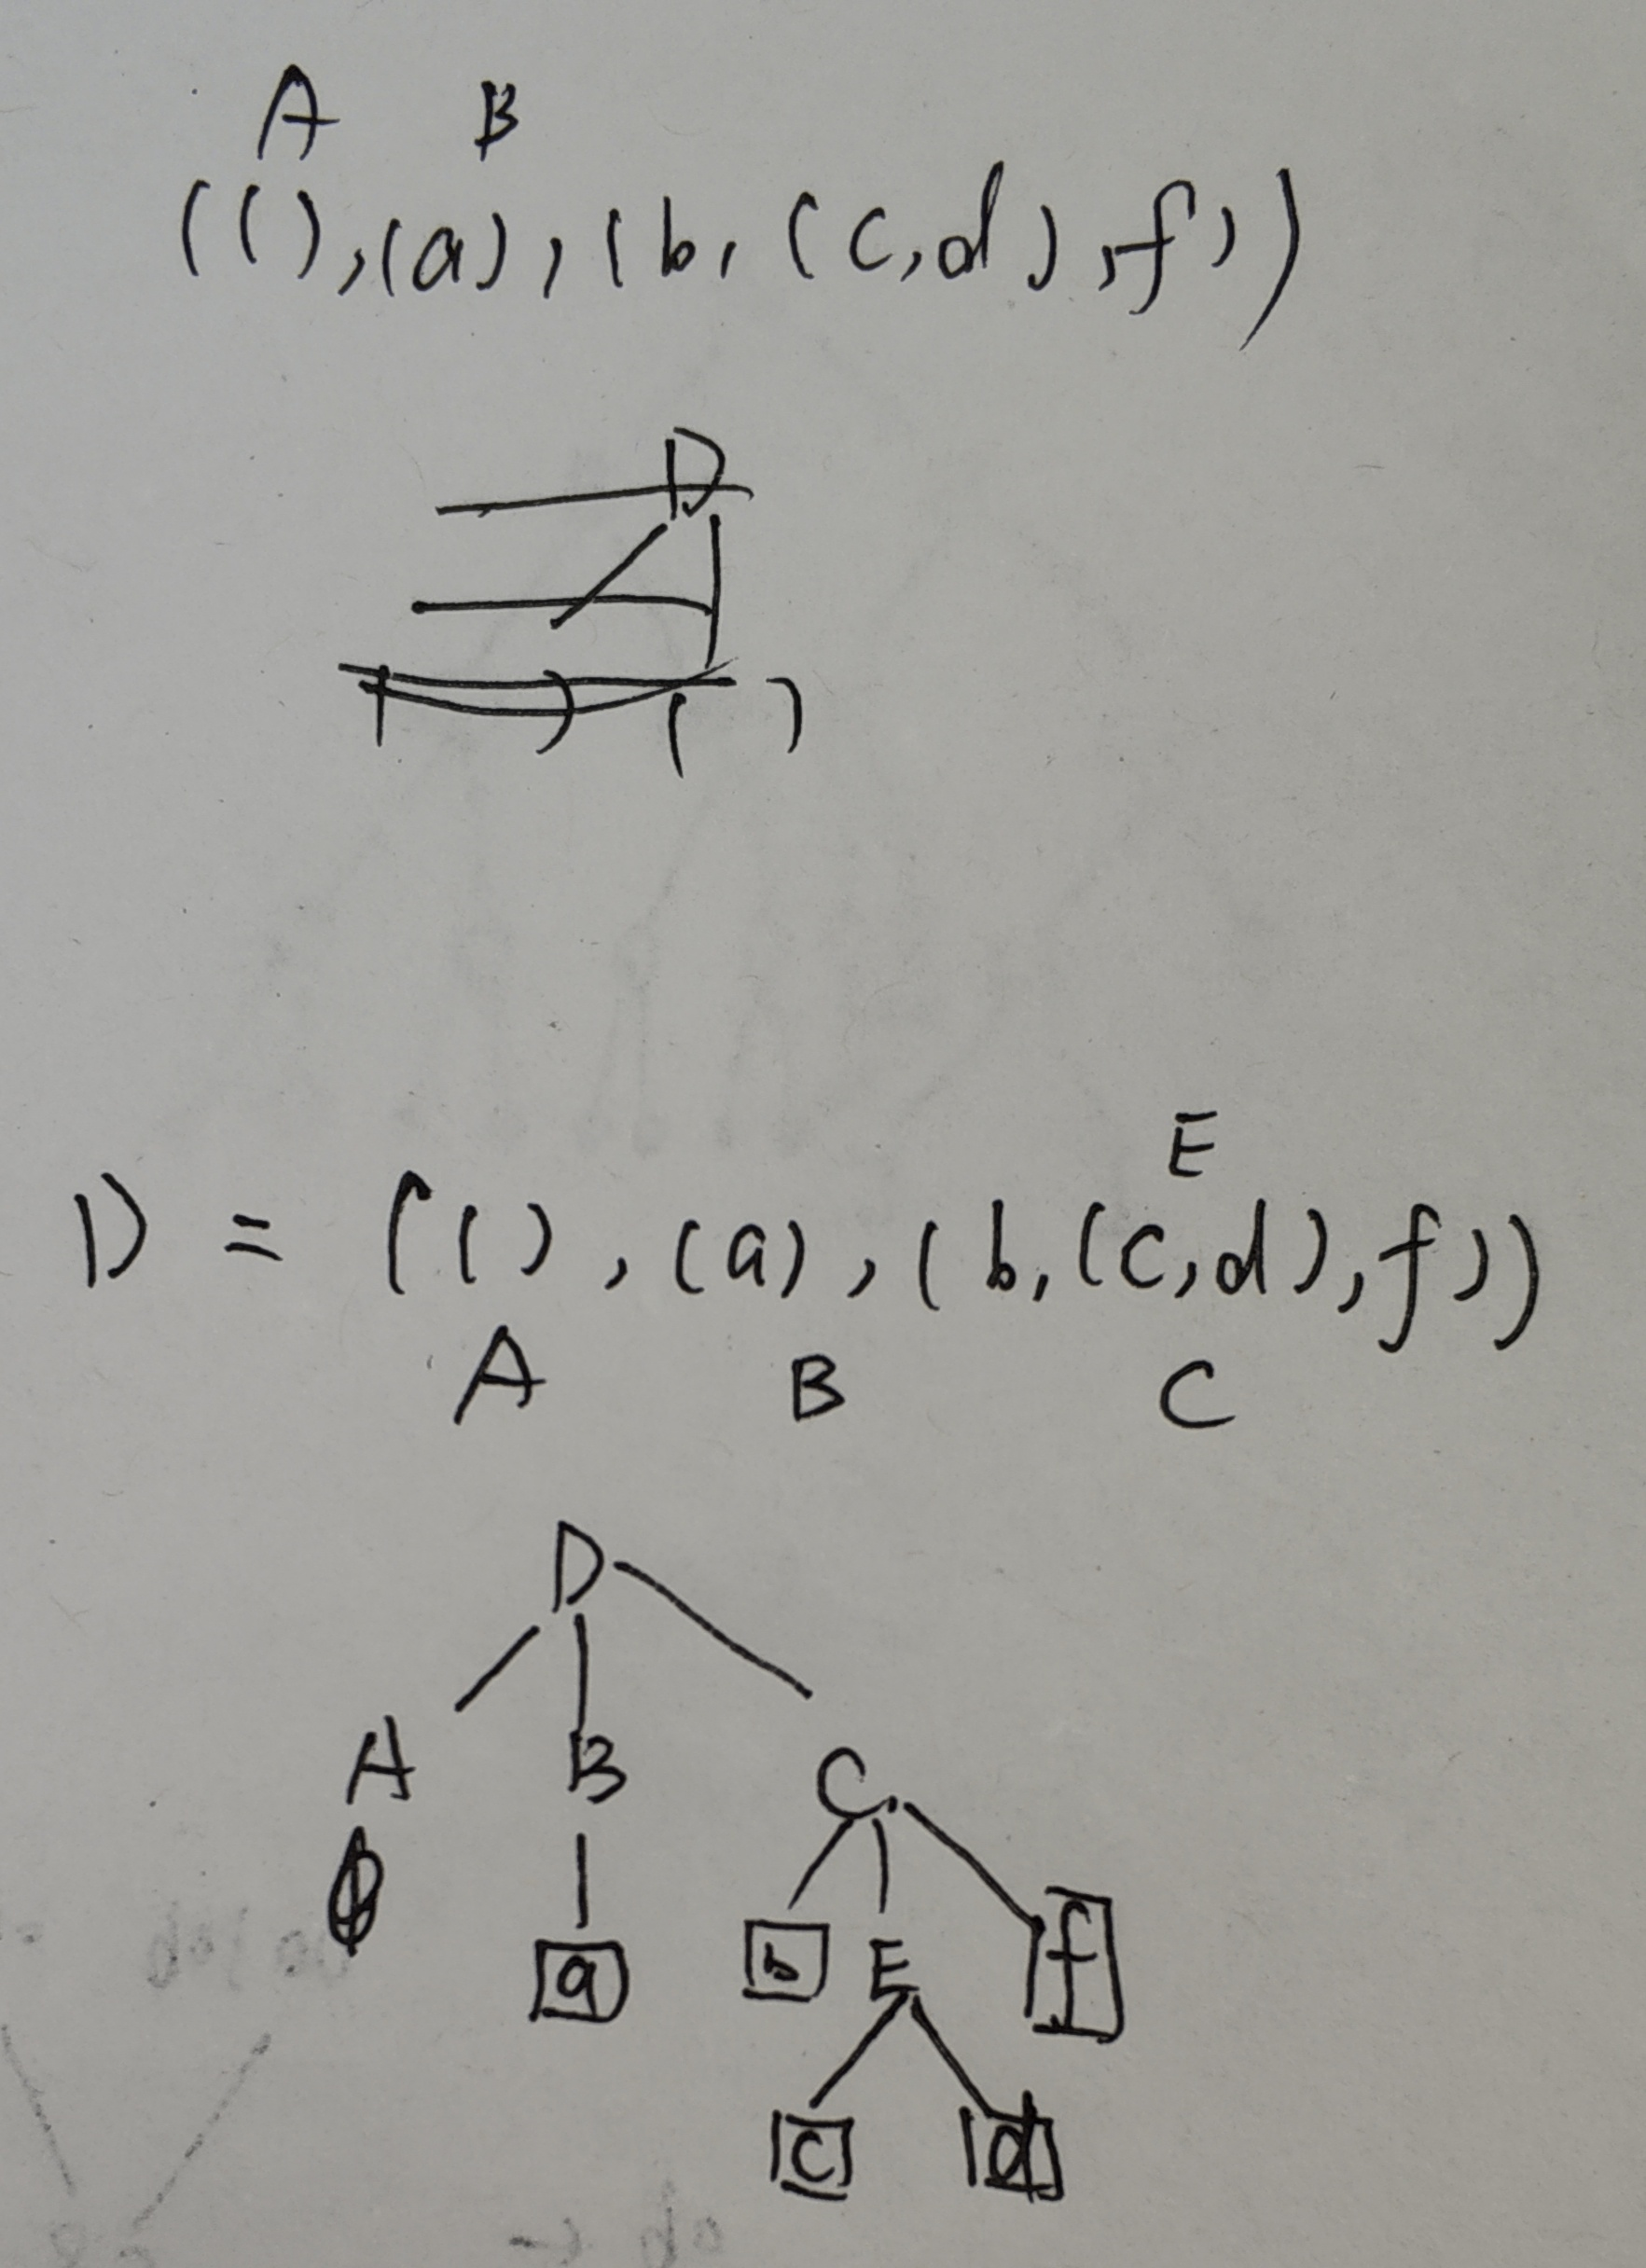
\includegraphics[scale=0.3]{example/chapter4/IMG_20181128_132004.png}
\end{figure}

求解深度参考链接\url{https://www.cnblogs.com/ciyeer/p/9040533.html}\newline
知道树的高度是4 但是最后一层是元素所以树的高度减去1就是广义表的深度。\newline

\subsection{2015年(5)}

\begin{lstlisting}[basicstyle=\small\ttfamily, caption={}, numbers=none]
已知广义表: A = (a,b), B = (A,A), C=(a,(b,A),B) 求下列运算的结果:tail(head(tail(C))) = (________)
\end{lstlisting}
解:\newline
C =(a,(b,A) ,B) \newline
  =(a,(b,(a,b)),((a,b),(a,b)) )\newline
Tail C =((b,(a,b)),((a,b),(a,b))) \newline
Head C' = (b,(a,b))\newline
Tail C'' = ((a,b))\newline
可知下划线上是  ((a,b)) - 即 (a,b)\newline